% !TEX TS-program = pdflatex
% !TEX encoding = UTF-8 Unicode

% This is a simple template for a LaTeX document using the "article" class.
% See "book", "report", "letter" for other types of document.

\documentclass[11pt]{article} % use larger type; default would be 10pt.
\setcounter{secnumdepth}{2}


\usepackage[utf8]{inputenc} % set input encoding (not needed with XeLaTeX)
\usepackage{float} % to place float images correctly

%%% Examples of Article customizations
% These packages are optional, depending whether you want the features they provide.
% See the LaTeX Companion or other references for full information.

%%% PAGE DIMENSIONS
\usepackage{geometry} % to change the page dimensions
\geometry{a4paper} % or letterpaper (US) or a5paper or....
% \geometry{margin=2in} % for example, change the margins to 2 inches all round
% \geometry{landscape} % set up the page for landscape
%   read geometry.pdf for detailed page layout information

\usepackage{graphicx} % support the \includegraphics command and options

% \usepackage[parfill]{parskip} % Activate to begin paragraphs with an empty line rather than an indent

%%% PACKAGES
\usepackage{booktabs} % for much better looking tables
\usepackage{array} % for better arrays (eg matrices) in maths
\usepackage{paralist} % very flexible & customisable lists (eg. enumerate/itemize, etc.)
\usepackage{verbatim} % adds environment for commenting out blocks of text & for better verbatim
\usepackage{subfig} % make it possible to include more than one captioned figure/table in a single float
% These packages are all incorporated in the memoir class to one degree or another...

%%% HEADERS & FOOTERS
\usepackage{fancyhdr} % This should be set AFTER setting up the page geometry
\pagestyle{fancy} % options: empty , plain , fancy
\renewcommand{\headrulewidth}{0pt} % customise the layout...
\lhead{}\chead{}\rhead{}
\lfoot{}\cfoot{\thepage}\rfoot{}

%%% SECTION TITLE APPEARANCE
\usepackage{sectsty}
\allsectionsfont{\sffamily\mdseries\upshape} % (See the fntguide.pdf for font help)
% (This matches ConTeXt defaults)

%%% ToC (table of contents) APPEARANCE
\usepackage[nottoc,notlof,notlot]{tocbibind} % Put the bibliography in the ToC
\usepackage[titles,subfigure]{tocloft} % Alter the style of the Table of Contents
\renewcommand{\cftsecfont}{\rmfamily\mdseries\upshape}
\renewcommand{\cftsecpagefont}{\rmfamily\mdseries\upshape} % No bold!
\newcommand{\pe}{PowerEnJoy }
\newcommand{\pecomma}{PowerEnJoy, }

%%% END Article customizations

%%% The "real" document content comes below...




\title{Requirements Analysis and Specifications Document (RASD)}
\author{Simone Mosciatti \& Sara Zanzottera}

\begin{document}
\maketitle
\newpage
\tableofcontents
\newpage



\subsection{Proposed System}

The proposed system features a client-server architecture, so it is divided into two parts: a frontend app for smartphones, which allows the users to use the service, and a backend system wich deals with all the operations and coordinates them. The backend also interact with the cars, that can be seen as a third part of the system.

\begin{figure}[H]
	\centering
	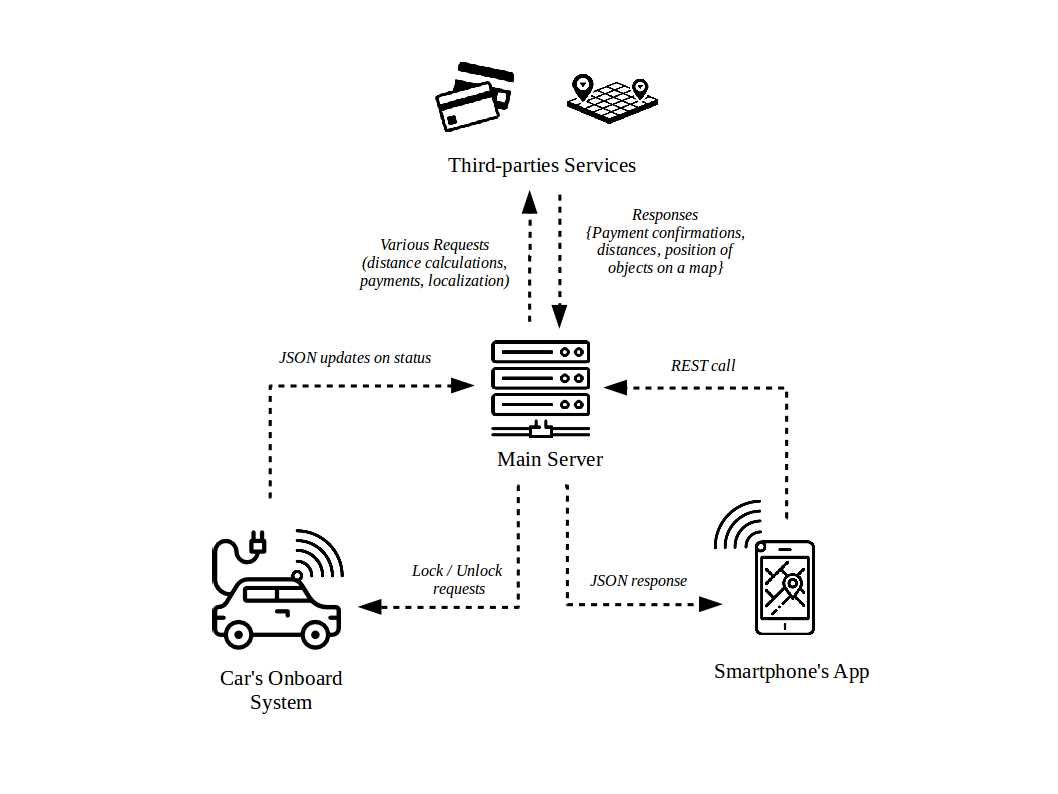
\includegraphics[width=1\textwidth]{proposed_system.png}
	\caption{Description of the proposed system.}
\end{figure}

\subsubsection{App Frontend}
The frontend is a thin app that relies on the smartphone's internet connections in order to work. Almost no operations can be performed with the app alone: all transactions are sent to the main server first, then processed and the result sent back to the app.

The app can be classified as a thin client.

\subsubsection{Centralized Backend}
The backend is the core of the system. Being able to process a lot of parallel operations, it can deal with all the requests coming from che clients ina reasonable amount of time (see Non Functionals Requirements). The backend is based on an MVC architecture and a REST API.

\subsubsection{Car's Onboard system}
The cars are equipped with an onboard system that monitors the status of the car, its location, and can send all the necessary informations to the main server. There won't be direct interactions between the car and the user's app.





\newpage
\section{Specific Requirements}

In this section we are going to illustrate the specific requirement of \pe.

We analyze the goals that the application should fullfill, then moving on functional and not functional requirements.

 \subsection{Goals}

\subsection{Domain Properties}

\subsection{Definitions,  acronyms,  abbreviations}
  	
  \begin{description}
  	\item[GPS]: Global Positioning System is a global navigation satellite system (GNSS) that provides location and time information in all weather conditions, anywhere on or near the Earth where there is an unobstructed line of sight to four or more GPS satellites.
  	\item[Frontend]
  	\item[Backend]
  \end{description}
  

\newpage
\section{Scenarios and Use Cases}

\subsection{Scenarios}

\subsection{Use Cases}


\newpage
\section{Alloy Model}

\newpage
\section{Hours}


\end{document}
